\chapter{绪\hspace{6pt}论}
\label{chapter:introduction}

\section{研究工作的背景与意义}
\label{sec:intro}
\subsection{研究背景}
\label{subsec:intro-background}

随着信息技术产业的高速发展,数字信息量呈爆炸式增长。国际数据资讯公司(IDC)\cite{IDC}于2020年公布的统计及预测报告\cite{DataReport2020}显示,每年新产生的数据量在2015年至2025年间以约26\%的复合年增长率增长,预计仅2025年创建的新数据数据量将高达175.8\,ZB(而2015年仅为18.2\,ZB)。新创建数据量的快速增长导致个人及企业面临的数据存储和管理成本快速上涨\cite{敖莉2010重复数据删除技术}。另一方面,在各类型存储系统所保存的数据中,高达60\%的数据都是冗余的。并且,随着时间的推移,这些冗余数据占总数据量的比例将进一步上升\cite{mcknight2006digital}。近年来,存储系统中数据高度冗余的特点得到越来越多研究人员的关注,利用该特点来节省存储空间、降低存储管理开销是成为热门研究课题。

重复数据删除(data deduplication)\cite{付印金2012重复数据删除关键技术研究进展, 敖莉2010重复数据删除技术,xia2016Deduplication,Paulo2014} 是一种粗粒度数据压缩技术。传统数据压缩针对小规模数据(例如同一文件内部),使用字节级重新编码以降低冗余;而重复数据删除作用的基本单位是数据块(通常为8KiB),通过比较来自相同和不同文件的数据块,为具有相同内容的数据块仅保存一份物理拷贝以节约存储空间。如图~\ref{fig:Deduplication-storage-pattern}所示,在支持重复数据删除的各类存储系统(统称为重复数据删除系统)中,重复数据删除后的任何数据块都被一个或多个文件引用,而每个文件则以指向这些数据块的指针的集合形式进行存储。重复数据删除可为主存和备份数据分别节省50\%\cite{meyer11}和98\%\cite{wallace12}的存储空间,可显著降低云存储厂商的存储及维护成本\cite{付印金2012重复数据删除关键技术研究进展}。由于能够有效地降低存储开销,重复数据删除技术非常适合为管理日益增长的海量数据节省成本。在工业界,Dell EMC Data Domain\cite{EMCDataDomain}、Avamar\cite{Avamar}、Veritas的NetBackup Appliances\cite{veritas} 以及Commvault的开放数据平台\cite{CommVault} 都是较为知名的重复数据删除应用产品;此外,各大云存储厂商(例如 Dropbox\cite{Dropbox}、Google Drive\cite{GoogleDrive}、百度网盘\cite{BaiduPan}等)也纷纷将重复数据删除技术应用于各自的云服务产品中,以提升经济效益\cite{harnik2010side}。  

\begin{figure}[!htb]
    \small
    \centering
    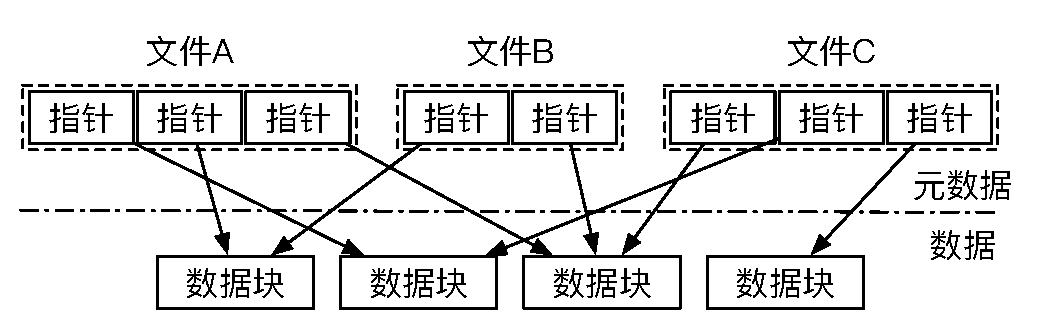
\includegraphics[width=0.75\textwidth]{pic/DedupSystemStorageMode.eps}
    \caption{重复数据删除系统的存储模式} 
    \label{fig:Deduplication-storage-pattern}
\end{figure} 

\textbf{本文重点关注面向云环境的重复数据删除}。图~\ref{fig:Cloud-based-deduplication-storage-logic}描述了云环境重复数据删除系统框架。云服务商维护哈希索引表,记录所有已存储数据块的哈希值。在重复数据删除过程中,用户使用云存储客户端计算目标数据块的哈希值;云服务商检查该哈希值是否存在于数据块索引表中,如果哈希值存在(即云端已有目标数据块的副本),则更新目标数据块的所有权信息并通知客户端无需传输该数据块,从而同时节省传输带宽和存储空间(这种重复数据删除方式称为源端重复数据删除(source-based deduplication))。然而,由于重复数据删除系统中任意重复数据块均只保留一个副本,任意一个数据块的泄露可能扩散影响到共用该数据块的所有文件。这种文件共用数据块的存储模式强调了数据块的敏感性。因此,如何保护重复数据删除后的数据的隐私,成为云存储服务商应用重复数据删除技术亟需解决的关键问题。

\begin{figure}[!htb]
    \small
    \centering
    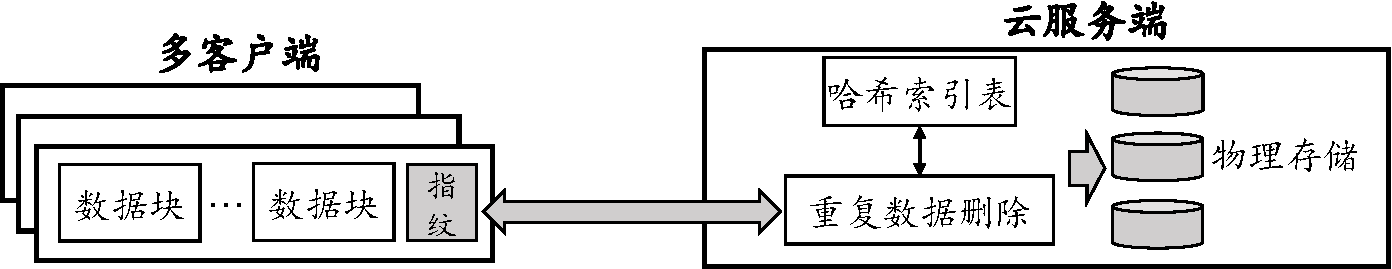
\includegraphics[width=\textwidth]{pic/Cloud-deduplication.pdf}
    \caption{云环境重复数据删除系统结构} 
    \label{fig:Cloud-based-deduplication-storage-logic}
\end{figure} 

近年来,研究者提出加密后重复数据删除\cite{bellare2013MLE}以保护重复数据删除过程中的数据安全。图~\ref{fig:Cloud-based-encrypted-deduplication-storage-logic}描述了加密后重复数据删除系统框架,其包括客户端和云服务端两个主要组成部分。为了防止云服务商获取外包数据内容,加密后重复数据删除系统在客户端部署消息锁加密(MLE:message-locked encryption)\cite{bellare2013MLE}以加密明文数据块(简称为明文数据块),同时确保重复数据删除仍然能够作用于密文数据块(简称为密文数据块)以节约存储空间。传统对称加密算法为每个客户端或每个数据块分配不同加密密钥,导致相同的明文数据块被加密为不同的密文数据块,无法通过重复数据删除进行冗余消除。消息锁加密的核心思路时基于数据块内容产生密钥(称为MLE密钥,例如MLE密钥为明文数据块的哈希值\cite{douceur2002reclaiming}),从而将相同明文数据块加密为相同的密文数据块,以兼容直接针对密文数据块的重复数据删除。现有消息锁加密采用服务器辅助密钥生成方式(称为服务器辅助消息锁加密(Server-aided MLE)
\cite{bellare2013DupLESS}),即部署第三方密钥服务器管理全局秘密,同时基于明文数据块哈希值以及密钥服务器的全局秘密共同生成MLE密钥,以防止攻击者针对MLE密钥实施离线暴力破解攻击。

\begin{figure}[!htb]
    \small
    \centering
    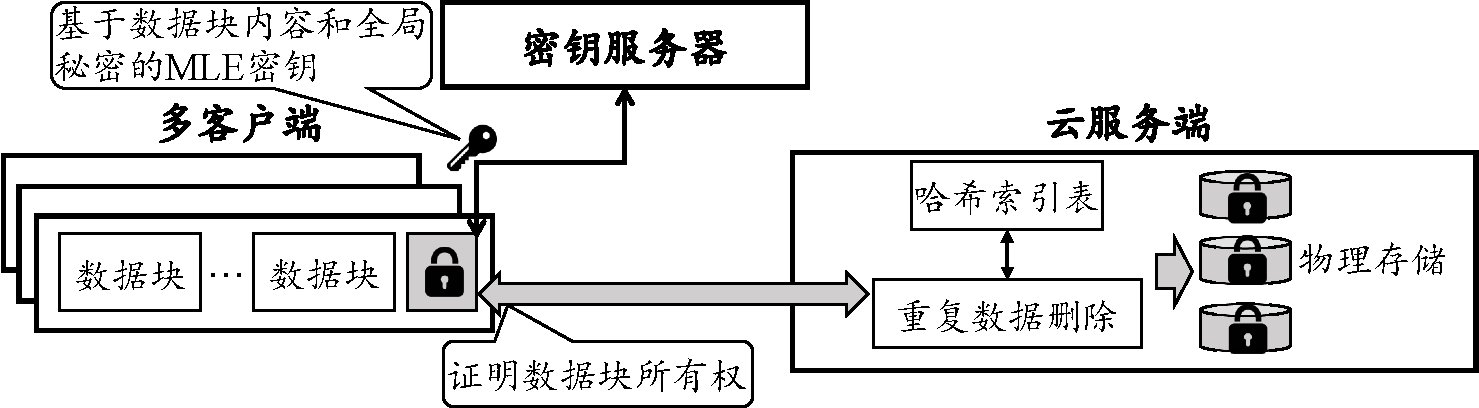
\includegraphics[width=\textwidth]{pic/Cloud-encrypted-deduplication-logic.pdf}
    \caption{面向云环境的加密后重复数据删除系统框架}
    \label{fig:Cloud-based-encrypted-deduplication-storage-logic}
\end{figure}

另一方面,重复数据删除受到伪造数据所有权的攻击威胁\cite{harnik10,mulazzani11}。由于云服务商仅基于收到的数据块哈希值判断客户端是否拥有相应数据块,恶意用户/客户端可以伪造任意密文数据块的哈希值,如果该密文数据块已在云端存储(即已发生重复数据删除),则恶意客户端无需传输密文数据块内容便可获得相应密文数据块的访问权限。为了防止伪造所有权攻击,加密后重复数据删除增加了所有权证明(proof-of-ownership)技术\cite{halevi11}:除了密文数据块的哈希值以外,云服务商要求客户端额外提交目标密文数据块的所有权证明(proof);云服务商首先基于证明验证该客户端是否真实且完整拥有相应密文数据块,然后再执行如前所述的重复数据删除过程。所有权证明技术的合理性在于,只针对客户端真实拥有(即具有完整访问权限)的密文数据块执行重复数据删除,从而避免非法访问其他客户端已在云端存储的内容。

\subsection{问题和动机}
\label{subsec:intro-problem}

现有面向云环境的加密后重复数据删除系统面临着系统效率低与安全性不足的双重挑战:

\subsubsection{系统效率} 
\label{subsubsec:intro-problem-performance}

在服务器辅助密钥生成过程中,现有加密后重复数据删除系统(图~\ref{fig:Cloud-based-encrypted-deduplication-storage-logic})须使用基于盲签名\cite{armknecht2015transparent,bellare2013DupLESS}的无记忆伪随机函数(OPRF:oblivious pseudorandom function)生成密钥\cite{bellare2013DupLESS},以防止密钥服务器获得明文块的哈希值。同时,为了实现所有权证明,系统须在云服务端维护Merkle哈希树,并基于哈希树验证客户端提交的证明信息\cite{halevi2011proofs}。本文指出,服务器辅助密钥生成和所有权证明的密码操作是加密后重复数据删除系统的主要效率瓶颈。

为了验证以上论断,本文基于图~\ref{fig:Cloud-based-encrypted-deduplication-storage-logic}框架和现有技术方案实现了加密后重复数据删除系统的基础原型。基础原型支持基于RSA\cite{bellare2013DupLESS}或BLS\cite{armknecht2015transparent}盲签名生成密钥,以及基于Merkle哈希树\cite{halevi2011proofs}或通用哈希(universal hash)\cite{xu2013weak}证明所有权(注:基于通用哈希的所有权证明方法\cite{xu2013weak}只能达到较低安全性)。

\begin{table}[!htb]
    \small
    \centering
    \begin{tabular}{@{}ccc@{}}
    \toprule
                           & 处理阶段/可选方案          & 处理时间(ms/MiB) \\ \midrule
                           & 数据分块               & 3.8          \\
    服务器辅助密钥生成              & RSA盲签名方案(BLS盲签名方案) & 40.7(488.3)  \\
    \multirow{3}{*}{所有权证明} & 数据加密               & 2.5          \\
                           & 哈希树方案(通用哈希方案)      & 27.0(7.2)    \\
                           & 重复数据删除             & 1.7          \\ \bottomrule
    \end{tabular}
    \caption{基础原型每个步骤处理1MiB数据的时间开销:括号内为可供备选的服务器辅助密钥生成方案和所有权证明方案,以及相应处理时间}
    \label{tab:intro-bottleneck}
\end{table}

表~\ref{tab:intro-bottleneck}展示了基础原型每个步骤处理1MiB数据的平均时间开销。服务器辅助密钥生成是最大效率瓶颈。如果采用基于Merkle哈希树的所有权证明方案,RSA盲签名和BLS盲签名分别占系统总开销的53.8\%和93.3\%。同时,所有权证明也是限制系统效率的重要因素,如果采用基于RSA盲签名的服务器辅助密钥生成方案,Merkle哈希树和(较低安全性的)通用哈希方案分别占系统总开销的35.7\%和9.5\%。

\subsubsection{安全隐患} 
\label{subsubsec:intro-problem-security}

现有支持数据块所有权证明技术的加密后重复数据删除依然不足以完全击败恶意客户端。在重复数据删除过程中,云服务商通知客户端传输或不传输密文数据块内容(\S\ref{subsec:intro-background}) ,实质上泄漏了“其他客户端是否已经存储相应密文数据块”的侧信道信息(side-channel information)。虽然所有权证明阻止了针对非授权密文数据块的重复数据删除,但不足以防止恶意客户端的侧信道攻击。例如,攻击者可以枚举所有可能的数据内容,并利用重复数据删除泄漏的侧信道信息实施推测内容攻击({\em learning-content attack})\cite{harnik10,zuo2018mitigating}。假设攻击者已知某个客户端持有目标文件且文件内容符合固定的公开格式(例如工资条、合同等模版化数据),致力于推断目标文件未公开的敏感内容(例如薪水金额)。攻击者枚举所有可能的未公开内容,并通过恶意客户端上传所生成的枚举文件。如果上传某个枚举文件时无需传输任何密文数据块,即可推断该枚举文件即为目标文件。此时,由于攻击者完全获得了所枚举文件的访问权限,仅检测所有权无法阻止推测内容攻击。

本文扩展现有工作\cite{harnik10,zuo2018mitigating}对推测内容攻击的场景分析,设计案例验证推测内容攻击的可行性。考虑Alice和Bob为应届毕业学生,同时收到某公司的雇佣合同。他们将各自合同备份至云端。假设Alice为攻击者,通过推测内容攻击推断Bob合同中的薪水和签字费。

\begin{table}[!htb]
    \small
    \centering
    \begin{tabular}{@{}cccc@{}}
    \toprule
    测试环境 & 上传次数                            & 上传流量(MiB)                       & 攻击时间(秒)        \\ \midrule
    局域网  & \multirow{2}{*}{841.0 $\pm$ 608.3} & \multirow{2}{*}{7.4 $\pm$ 5.4} & 105.0 $\pm$ 76.1 \\
    阿里云  &                                 &                                 & 475.5 $\pm$ 339.8 \\
    \bottomrule
    \end{tabular}
    \caption{推测内容攻击开销:以上结果包含十次测试数据基于T分布的95\%置信区间}
    \label{tab:intro-LRI-verify}
\end{table}

为了实现以上推测内容攻击案例,本文基于Google合同模版\cite{GoogleOffer},更改其中姓名、年薪(假设为6K的倍数\cite{harnik10},介于204K和804K之间)和签字费(假设为10K的倍数,介于300K和600K之间)以生成Alice和Bob的合同,每个合同约占18.5KiB。本文随机生成Bob的薪水和签字费,并通过基于图~\ref{fig:Cloud-based-encrypted-deduplication-storage-logic}设计实现的基础原型将Bob的合同存储至服务端。令Alice基于自身合同作为内容模版,枚举Bob所有可能的薪水和签字费,以实施推测内容攻击。本文分别在本地局域网(客户端、密钥服务器和服务端均部署在具有10\,Gb/s网速的本地实验环境)和阿里云(在本地部署客户端和密钥服务器,在阿里云部署服务端)实现上述攻击。Alice需上传大约841份伪造合同,消耗7.4MiB网络流量(包括传输非重复密文数据块和元数据),在局域网和阿里云环境中推断Bob的隐私信息分别只需105.0秒和475.5秒。

\subsection{研究内容概述}
\label{subsec:intro-content}

本文指出,现有加密后重复数据删除使用纯软件实现的密码算法保障数据安全,但是,由于密码算法计算开销大、安全防护不完整,导致当前的重复数据删除系统存在效率和安全方面的不足。因此,本文拟开展基于硬件可信执行环境的安全重复数据删除研究,意图通过硬件实现的可信执行环境(TEE:trusted execution environment)优化/改变现有基于纯软件的重复数据删除方法思路,进而克服现有研究的不足。具体的,TEE是一组软硬件结合的系统组件,可为应用程序提供必要的基础设施和运行资源,同时为内部代码的安全执行提供机密性和完整性保证\cite{OMTP}。各大软硬件厂商均推出了各自的TEE实现方案,包括TrustZone\cite{trustzone}、Intel SGX\cite{sgx,sgx2}、AMD SEV\cite{AMDSEV}、Apple Secure Enclave\cite{AppleSecureEnclave}、Google Titan\cite{GoogleTitan}等。为了避免硬件依赖,本文的系统设计并不基于某一具体的TEE解决方案,统一使用“安全区”指代TEE实现的具有隔离条件和安全保障的程序执行环境。本文的核心方法是,在安全区内执行面向明文数据的敏感操作,以基于硬件的保护方式替代传统基于纯软件实现的复杂密码算法,从而保持安全性并提高系统效率。

针对现有面向云环境的加密后重复数据删除存在密钥生成效率低、所有权证明计算复杂、易于遭受推测内容攻击等不足。本文拟改进现有的加密后重复数据删除方法,提出:

\begin{enumerate}
    \item 基于TEE的轻量级密钥生成技术,以提升服务器辅助密钥生成的效率和可扩展性。
    \item 基于TEE的高效所有权证明技术,以提升所有权证明效率。
    \item 基于TEE的扩展所有权证明技术,以进一步防止推测内容攻击(现有所有权证明技术不足以防止推测内容攻击,见\S\ref{subsubsec:intro-problem-security})。
\end{enumerate}

\subsection{研究意义}
\label{subsec:intro-meaning}

在学术界,自收敛加密\cite{douceur2002reclaiming}提出以来,安全重复数据删除已有20余年研究历史,但由于一些本质问题(例如效率、侧信道攻击、密钥管理等,见\S\ref{subsec:intro-problem})未能得到妥善解决而难以落地推广;并且,目前的学术研究聚焦于解决某一方面本质问题,同时以牺牲另一方面性能为代价(\S\ref{subsubsec:intro-problem-performance})。本文的学术研究意义在于,\textbf{突破现有安全重复数据删除方法局限,同时妥善解决效率、安全、存储多个本质问题,推动安全重复数据删除理论到实践的转化。并且,本文作为TEE在数据存储领域的应用范例,所提出的系统和方法对TEE在其他领域研究具有参考价值。}

在工业界,本文研究的安全、效率、成本问题是云服务商关注的焦点问题。一方面,数据安全隐私和服务使用体验,是决定用户是否选择云服务的关键因素;另一方面,重复数据删除有助于降低设备购置和维护成本,提升云服务商的经济效益。因此,本文的应用实践价值在于,\textbf{在服务商关注的安全、效率、成本维度,研究的系统和方法将全面领先于现有基于纯软件的安全存储解决方案,将推动未来基于TEE的云存储架构,对促进云服务产业发展具有积极意义。}

\section{国内外研究历史与现状}
\label{sec:compare}

\subsection{加密后重复数据删除}
\label{subsec:compare-deduplication}

\S\ref{subsec:intro-problem}指出了加密后重复数据删除系统面临的系统效率、安全隐患方面的不足,接下来将综述现有的针对性解决方法及其与本文研究内容的区别。

\subsubsection{系统效率}
\label{subsubsec:compare-deduplication-performance}

为了解决服务器辅助密钥生成效率瓶颈,SecDep\cite{zhou2015secdep}提出生成粗粒度的文件级MLE密钥,并针对不同用户之间的相同数据使用文件级重复数据删除;本文提出了基于相似性密钥生成方法\cite{qin17},为若干个连续明文块生成基于代表性明文块(例如其中具有最小哈希值的明文块)的MLE密钥,用以加密其中的每个明文块。以上方法均是通过减少MLE密钥生成次数来解决效率问题,但导致部分相同明文块被加密为不同密文数据块而无法被删除。本文研究的基于TEE的轻量级密钥生成技术将提升单次密钥生成速率,同时允许删除所有数据块级冗余;研究的加密前重复数据删除方法无需通过服务器辅助方式生成密钥。
在所有权证明方面,研究者通过降低安全性提升效率\cite{xu2013weak,pietro12},但是,本文研究的基于TEE的扩展所有权证明技术将同时提升所有权证明的安全性和效率。

\subsubsection{安全隐患}
\label{subsubsec:compare-deduplication-security}

本文总结分析以下几种防御推测内容攻击的方案,这些方案均可保护源端重复数据删除中可能泄露的重复数据删除信息。

\begin{enumerate}
    \item \textbf{目标端重复数据删除(target-based deduplication)}\cite{harnik10}强制客户端传输所有密文数据块后在服务端删除重复密文数据块,使得重复数据删除过程向客户端完全隐藏。
    \item \textbf{随机阈值重复数据删除(randomized-threshold deduplication)}\cite{harnik10}为每个密文数据块分配一个随机阈值,如果密文数据块被上传次数超过阈值,则执行源端重复数据删除(\S\ref{subsec:intro-background}),否则执行目标端重复数据删除。由于系统为每个数据块设立的阈值完全随机,恶意客户端无法确定该数据块被上传次数。
    \item \textbf{两阶段重复数据删除(two-stage deduplication)}\cite{li2015cdstore}针对来自同一客户端的密文块采取源端重复数据删除,而对来自不同客户端的密文块采取目标端重复数据删除。该防御机制的原理是恶意客户端仅能获得其自身所有数据块的重复数据删除信息。
    \item \textbf{随机冗余数据块传输方案(RRCS)}\cite{zuo2018mitigating}工作在文件级别,其通知每个客户端传输上传文件中的多个随机的重复数据块,以及相应的非重复数据块,这样攻击者无法在重复和非重复的文件之间区分传输的数据块个数。 
\end{enumerate}

以上方法均须传输全部(目标端重复数据删除)或部分(随机阈值重复数据删除,两阶段重复数据删除和随机冗余数据块传输方案)重复数据,增加网络资源和服务端处理开销。本文研究的基于TEE的扩展所有权证明技术兼容源端重复数据删除而无需传输任意重复数据块。 

\subsection{基于TEE的安全应用}
\label{subsec:compare-tee}

TrustZone和SGX是目前应用最广泛的TEE解决方案\cite{pinto19}。TrustZone是ARM CPU指令集的安全扩展,主要应用于低功耗移动平台以保护敏感应用程序的执行逻辑\cite{rubinov2016automated}、用户输入口令\cite{ying2018truz},以及监控安全区以外的程序执行\cite{azab2014hypervision}。SGX是Intel CPU指令集的安全监控扩展,已被广泛用于加强不同应用系统的安全性,包括比特币\cite{matetic19}、文件系统\cite{ahmad2018OBLIVIATE,shinde20}、外包数据库\cite{eskandarian17,priebe18,sun21}、键值存储\cite{mishra2018Oblix,bailleu2019SPEICHER,kim19,bailleu2021Avocado}和数据分析平台\cite{schuster15, zheng2017Opaque, bowe2020ZEXE}等。

TEE已被广泛用于保护存储系统。PESOS\cite{krahn18}使用SGX强化对象存储中的访问策略。OBLIVIATE\cite{ahmad2018OBLIVIATE}增强了基于SGX的文件系统对特权侧信道攻击的安全性。EnclaveDB\cite{priebe18}和ObliDB\cite{eskandarian19}基于SGX保护外包数据库免受信息泄露威胁。NEXUS\cite{djoko2019NEXUS}通过SGX对不受信任的云存储启用细粒度的访问控制。在性能方面,Harnik等人\cite{harnik18}提出了降低基于SGX系统的性能开销的指南。ShieldStore\cite{kim19}实现特定于应用程序的数据管理以减少安全区内存开销。SPEICHER\cite{bailleu2019SPEICHER}则是一个基于SGX及LSM树(Log-structured merge-tree)\cite{LSMT}的键值存储系统,具有高效的I/O操作能力。\textbf{然而,以上所有研究均未考虑重复数据删除。}

Dang等人\cite{dang2017Privacy}提出了基于代理的加密后重复数据删除协议,用于低网络资源开销的加密后重复数据删除,但这些协议没有解决密钥生成性能开销,也没有实现相关原型系统。SPEED\cite{cui2019SPEED}利用重复数据删除来提高SGX的计算效率,但本文使用安全区提高了加密后重复数据删除的性能。其他研究使用云端安全区实现数据块所有权验证\cite{you2020Proofs}和基于文件的加密后重复数据删除\cite{fuhry20},而本文使用客户端安全区进行有效的数据块所有权证明生成并支持更细粒度的基于数据块的重复数据删除。SeGShare\cite{fuhry2020segshare}在服务端部署安全区实现文件级重复数据删除,但无法删除相似文件中的相同数据块。S2Dedup\cite{miranda2021S2Dedup}在服务端部署安全区以重加密来自不同客户端的密文数据块,并在安全区外执行针对重加密后密文数据块的重复数据删除,但是,由于所有数据块的重复数据删除均需进出安全区,S2Dedup产生了严重的CPU上下文切换开销(context-switching overhead)\cite{weisse2017regaining}。

\section{本文的主要贡献与创新}

\begin{enumerate}
    \item \textbf{系统性研究如何使用TEE改进重复数据删除,为后续TEE应用起到一定启发作用。}
    尽管已有少量工作提出基于TEE的重复数据删除方法,但这些工作或者只支持粗粒度文件级重复数据删除\cite{fuhry2020segshare},或者由于持续访问安全区外索引导致巨大环境切换开销\cite{miranda2021S2Dedup}。本项目明确了如何使用TEE改进现有加密后重复数据删除的密钥生成和所有权证明,以及实现对推测内容攻击的防御,并提供系统以论证实用性。本项目所提出的系统和方法对TEE在其他领域研究具有参考价值。
    \item \textbf{研发高效实用的加密前和加密后重复数据删除原型系统,推动安全重复数据删除理论到实践的转化。}
    本项目研发的原型系统均能解决服务商关注的安全、效率、成本问题,并全面领先于现有基于纯软件的存储解决方案,推动安全重复数据删除落地实践。
\end{enumerate}

\section{本论文的结构安排}

本文的其余部分安排如下:第二章将介绍本文中使用的相关概念及背景知识,第三章将介绍本文针对加密后重复数据删除系统效率进行的研究,第四章将介绍本文针对推测内容攻击安全威胁的防御进行的相关研究,最后第五章对本文的研究工作进行总结。